\documentclass[12pt]{article}
\usepackage{graphicx}
\usepackage{fullpage}
\usepackage{float}
\usepackage[symbol]{footmisc}
\graphicspath{{../images/}}
\usepackage{titlesec}% http://ctan.org/pkg/titlesec
\titleformat{\section}%
  [hang]% <shape>
  {\normalfont\bfseries\Large}% <format>
  {}% <label>
  {0pt}% <sep>
  {}% <before code>
\renewcommand{\thesection}{}% Remove section references...
\renewcommand{\thesubsection}{\arabic{subsection}}%... from subsections

\title{The Digital Age}
\author {
Kevin Yu
}

\begin{document}
\maketitle

\begin{abstract}
We study techniques of digital sampling and data analysis in order to demonstrate methods by which we can manipulate and study signals in both the time and frequency domains. We experiment with violating the Nyquist criterion and find that we cannot adequately represent signals with frequency components faster than half the sample rate. Additionally, we compare  heterodyne mixing with both with an analog DSB mixer and a digital SSB mixer, which allows us to convert a signal of frequency $\omega$ to a much lower frequency $\delta$ by mixing it with a local oscillator driven at a frequency $\omega \pm \delta$. We find that both methods produce comparable results when a Fourier filter is applied to the output. Finally, we use the ROACH's parallel processing powers to implement an eight tap FIR filter to create a digital $5/8$-band filter, which we find is not capable of replicating an \textit{ideal} filter shape but can come close with many samples. Figures and code can be found online at http://github.com/kevinyu/astro121.git. 
\end{abstract}

\section{Introduction}
In this lab, we learn the advantages and limitations of digital sampling and mixing, as well as methods of analyzing the spectral compsition of signals. Digital sampling is inherently limited by the need to translate a continuous signal's characteristics into discrete values that can be understood by a computer, which represents measurements in terms of binary \texttt{1}'s and \texttt{0}'s. Thus, there are trade-offs at every turn---for example, turning up your sampling rate will improve the shape of your waveform, but your computer's memory will fill up faster and you will not be able to sample for as long.

Luckily, knowing the limitations of digital sampling also allows us to determine ways in which we can save time/energy/memory without losing important information about the radio signals we are trying to study. In cases where we are dealing with frequencies much greater than can be handled by our equipment, we will want to use heterodyne mixing to shift the signal to a much lower frequency. We can then use tools such as discrete fourier transforms and digital filters to futher manipulate our signal to extract the underlying information we are looking for.


% In the first section of this report, I discuss methods of Fourier analysis---in particular using discrete Fourier transforms, or DFTs---which I will use throughout the lab to uncover the frequency composition of digital waveforms. In the section section, we investigate digital sampling and in particular the Nyquist criterion. In the third section, we experiment with heterodyne mixing, both in analog and in digital. Finally, in the finaly section we use these techniques and an FIR filter to create a digital down converter that mixes a signal with a local oscillator and filters the signal digitally.

\section{Methods and Results}

\subsection{Fourier Analysis}
The Fourier Transform, defined as
\begin{eqnarray}
\hat{f}(\omega) = \int_{-\infty}^{+\infty}f(t)e^{i\omega t} dt \label{eq:continuousfourier}
\end{eqnarray}
is the basic tool for analyzing a signal in both the time and the frequency domains. It allows one to decompose a signal into its Fourier components to see what frequencies it is ``made of".

When dealing with digitally sampled data, however, we can no longer use the integral in Eq. \ref{eq:continuousfourier}. For one, we are dealing with discretely sampled points, which means we need to use a summation instead of an integral. Additionally, we cannot take samples from $t=-\infty$ to $+\infty$---and even if we could, it would already be too late to start. In the case where we can only sample at a finite rate and for a finite period of time, the integral becomes the following summation:
\begin{eqnarray}
\hat{f}(\omega) = \frac{1}{N\Delta{t}}\sum_{n=1}^{N} f_n e^{j\omega n \Delta{t}} \Delta{t}
\end{eqnarray}
in which $N$ is the total number of sampled data points and $\Delta{t}$ is the timestep between samples $\left( 1/\nu_{samp} \right)$.

The na\"{i}ve implementation of this algorithm---which loops through frequencies in the range $-\frac{1}{2\Delta{t}}$ to $\frac{1}{2\Delta{t}}$ in steps of $\frac{1}{\Delta{t}}$---runs in $O\left(n^2\right)$ time, and thus is not suited to large datasets. However, in this lab I will use the more efficient \texttt{fft} (Fast Fourier Transform) algorithm for computing discrete Fourier transforms, provided by Python's scientific computing package NumPy. This algorithm's running time scales as $O\left( n \log_2(n) \right)$ and thus is suitable for large datasets.

Figures in the upcoming sections that contain plots of a power spectrum are created by first computing the \texttt{fft} of the waveform of interest, taking the magnitude of the complex output (using Python's \texttt{abs} function), and squaring the resulting values.

\subsection{Nyquist Frequency}
One of the most important concepts in digital sampling is the Nyquist criterion, which specifies the minimum frequency at which it is possible for a digitally sampled waveform to accurately reproduce the frequency composition of the actual signal. The Nyquist criterion can be put in this way: for a particular sample rate $\nu_{samp}$, only signal frequencies at or below the Nyquist rate
\begin{eqnarray}
 \nu_{nyquist} = \nu_{samp} / 2 \label{eq:nyquist}
\end{eqnarray}
can be captured by the sample. The reason for this is fairly intuitive; if one samples points separated by a time $\Delta{t}$, then any fluctuations in the signal that occur between the two samples will not be observed. To see a fluctuation in the signal, at least two points per period (one ``high" and one ``low") must be taken---this statement is equivalent to Eq.\ref{eq:nyquist}.

Failure to satisfy the Nyquist criterion will result in \textit{aliasing}, in which the sampled waveform appears to depict a slower frequency and possibly opposite phase to the original signal. An artistic interpretation of this phenomenon is shown in Figure \ref{fig:aliasing}.
\begin{figure}[H]
\center{
  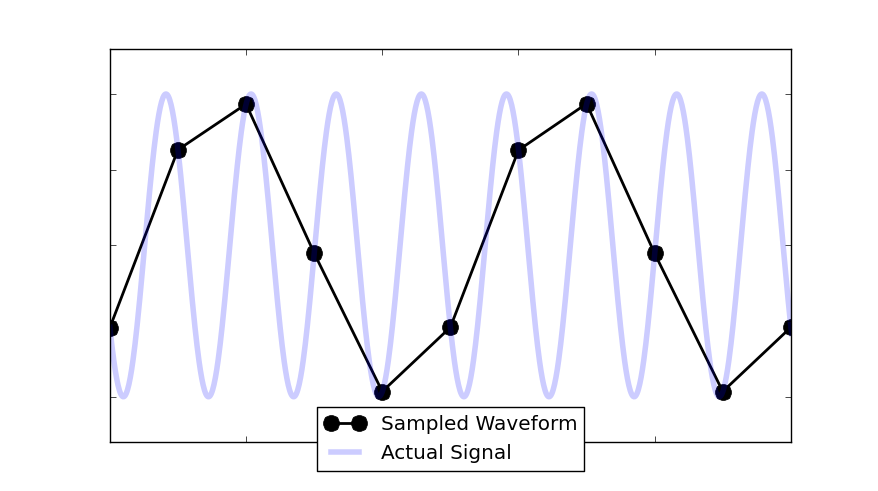
\includegraphics[width=400px]{aliasing}
}
\caption[SODUMB]{An example of aliasing. Because the sample rate is not fast enough to capture the high frequency information in the signal, the result appears to be of a slower frequency.}
\label{fig:aliasing}
\end{figure}

To demonsrate the effects of sampling above the Nyquist frequnecy, we use the Pulsar sampler card to take digital waveforms of incoming sine waves produced by the SRS Signal Generators. We fix our sampling rate at $\nu_{samp} = 10$ kHz\footnote{This is safely below the Pulsar's maximum sampling rate of $10$ MHz} so that the Nyquist frequency is $\nu_{nyquist} = 5$ MHz.

The sampled waveforms for signal frequencies ranging from $1$ kHz to $9$ kHz are shown in Figure \ref{eq:nyquist}. The corresponding power spectra from these sampled waveforms are shown in the right column.

\begin{figure}[H]
\center{
  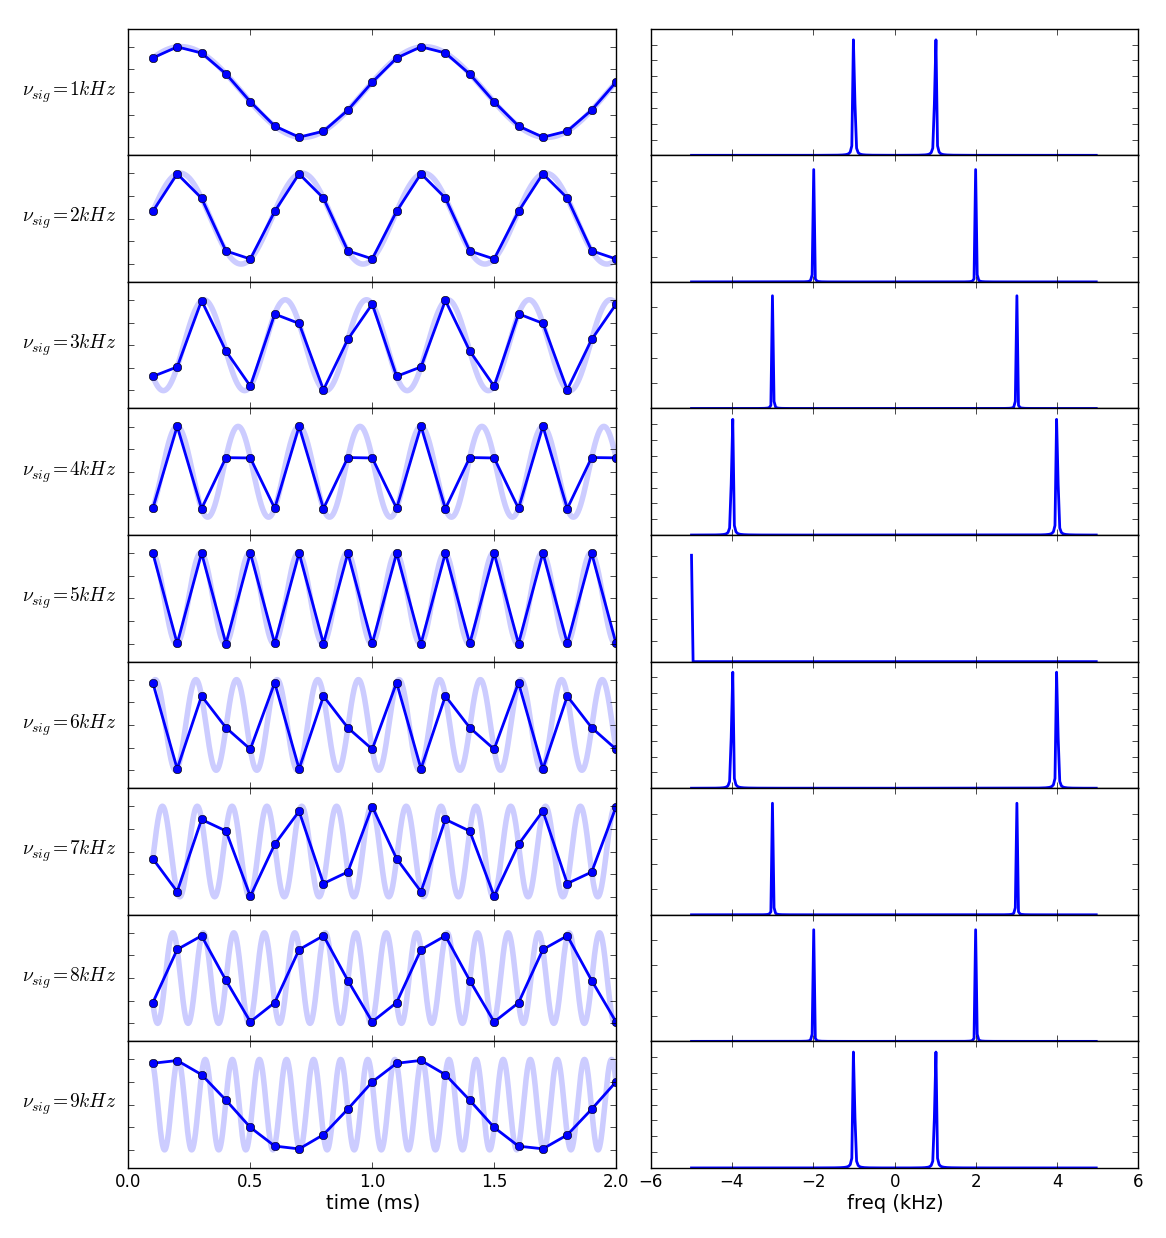
\includegraphics[width=460px]{nyquistsampling}
}
\caption[SODUMB]{Left: Time domain representation of sampled waveforms, with interpolation, sampled at $10$ kHz. The frequency of the original signal is shown on the left. A representation of the actual signal is overlayed in a lighter shade. Aliasing can be seen for signal frequencies greater than $\nu_{nyquist}=5$ kHz. Right: The corresponding power spectrum for sampled waveforms. For signal frequencies greater than the Nyquist rate, the observed frequencies are the actual frequencies reflected over $\nu_{nyquist}$. The power spectrum for $\nu_{sig}=5$ kHz is missing a spike at $+5$ kHz due to the nature of the \texttt{fft} program used, which is asymmetric around zero in that it omits the final frequency point on the positive side; the $5$ kHz frequency does, however, exist in the sampled waveform.}
\label{fig:nyquist}
\end{figure}

As can be seen from the time domain representation of our sampled waveforms in Figure \ref{eq:nyquist}, the signals slower than the Nyquist rate---from $1$ kHz to $4$ kHz---are all represented accurately in terms of their frequency. Though the interpolated waveforms appear jagged, the underlying sinusoidal shape and frequency of the signal are clearly visible. Additionally, the peaks in the power spectrum correspond well with the true frequency of its signal. Positive and negative spikes at the signal frequency are seen due to the signal only being real-valued, consisting of both an $e^{j\omega t}$ and $e^{-j\omega t}$ components.

At $5$ kHz, which is exactly the Nyquist rate, the sampled waveform is a series of ``high" and ``low" values, both staying at consistent levels. This is because the incoming signal is sampled \textit{exactly} twice per period, at exactly the same point in the sinusoid's cycle each time. Though the sampled points lack detail, the underlying $5$ kHz frequency is still clear in both the time domain representation and the fourier spectrum. However, we must be careful for this case; we got lucky that we sampled at approximately the top and bottom of the signal. If we had started sampling just a quarter period too late, we would only see a flat signal; we would still sample twice per period, but only at the points where the signal is crossing zero! We can conclude that although the Nyquist frequency gives us a minimum sampling frequency, we are better off sampling at least a little bit faster.

Finally, the most interesting results are for the cases in whih we violate the Nyquist criterion at signal frequencies greater than $5$ kHz. For signal frequencies $6$ kHz to $9$ kHz, we no longer see spikes at the expected frequencies in the power spectrum but instead at the expected frequencies \textit{reflected across} $\nu_{nyquist}$. When we look at the waveform in the time domain, it is clear that the sampled version of the signals look slower than they actually are.  Additionally, these sampled waveforms violating the Nyquist criterion appear to have a $180^\circ$ phase shift relative to the signal's actual phase; this can be seen by noticing that if the actual signal begins with a downward slope, the sampled waveform begins with an upward slope, or vice versa.

\subsection{Mixing} 

A local oscillator, or LO, is a signal used to convert an incoming signal to a different frequency through the process of mixing. When we \textit{mix} two signals, $f$ and $g$, we multiply them in the time domain, which is equivalent to convolving them in the Fourier, or frequency, domain.

When dealing with radio signals, our equipment may not be suited to the higher frequencies. If the frequency of interest is larger than our equipment is capable of handling, we can use heterodyne mixing to shift the signal to a lower frequency where it can be appropriately analyzed.

When we mix a real-valued signal of frequency $\nu_{sig}$ with a local oscillator of the form $e^{j 2\pi \nu_{LO} t}$, we will see the following frequency components in the spectrum of the output, which are calle d the intermediate frequencies (IF). They are:
\begin{eqnarray}
\nu_{IF} = \nu_{LO} \pm \nu_{sig}
\end{eqnarray}
if our local oscillator is only real-valued, consisting of both $e^{j 2\pi \nu_{LO} t}$ and $e^{-j 2\pi \nu_{LO} t}$ components, our intermediate frequencies are:
\begin{eqnarray}
\nu_{IF} = \nu_{LO} \pm \nu_{sig},\ -\nu_{LO} \pm \nu_{sig}
\end{eqnarray}
In order to convert a high frequency signal of frequency $\nu$ to a much slower frequency $\delta$, we can mix the signal with a local oscillator of frequency $\nu_{LO} = \nu + \delta$. This will result in intermediate frequencies of 
\begin{eqnarray}
\nu_{IF} = \delta,\ 2\nu + \delta \label{eq:bands}
\end{eqnarray}
From here, we can apply a filter to isolate the frequency component at $\delta$. 


\subsubsection{Analog Mixing (DSB)}
To demonstrate a heterodyne mixer, we first use an analog mixer, the ZAD-1, to mix a signal and local oscillator---each generated by one of the SRS Signal Generators. We choose our $\nu_{LO}$ to be $2$ MHz. Using this LO frequency, we first mix it with a signal of frequency $2.1$ MHz, and the second time with a signal of frequency of $1.9$ MHz. In both cases, the $\delta$ is $0.1$ MHz. 

Our expected intermediate values are the following table, keeping in mind the fact that both signal generators only produce real-valued signals:

\begin{center}
  \begin{tabular}{c | c | c | c }
    $\nu_{LO}$ & $\nu_{sig}$ & $\nu_{LO} \pm \nu_{sig}$ & $-\nu_{LO} \pm \nu_{sig}$ \\
    MHz & MHz & MHz & MHz \\ \hline
    2.0 & 2.1 & -0.1, 4.1 & -4.1, 0.1 \\
    2.0 & 1.9 & 0.1, 3.9 & -3.9, -0.1 \\
  \end{tabular}\\
\end{center}

Looking at the positive $\nu_{LO}$ frequencies (it is symmetric for the negative ones), we see that the output will be split into a lower sideband---$\nu_{LO} - \nu_{sig}$---and an upper sideband---$\nu_{LO} + \nu_{sig}$. Thus, we have a double sideband (DSB) mixer. A single sideband (SSB) mixer would require mixing with pure sinusoids of the form $e^{j\omega t}$, which have both a real and imaginary part. With a complex sinusoid, we would be able to eliminate one of the two sidebands.

To sample the output of our analog heterodyne DSB mixer, we use the Pulsar card and sample at a rate of $10$ MHz, the maximum frequency the Pulsar will sample at. We collect $N=16384$ data points, thus for each waveform we sample for $N*\Delta{t}$, or $1.6$ ms. Figure \ref{fig:analogmixing_spectrum} shows the power spectrum of the analog mixer output.

\begin{figure}[H]
\center{
  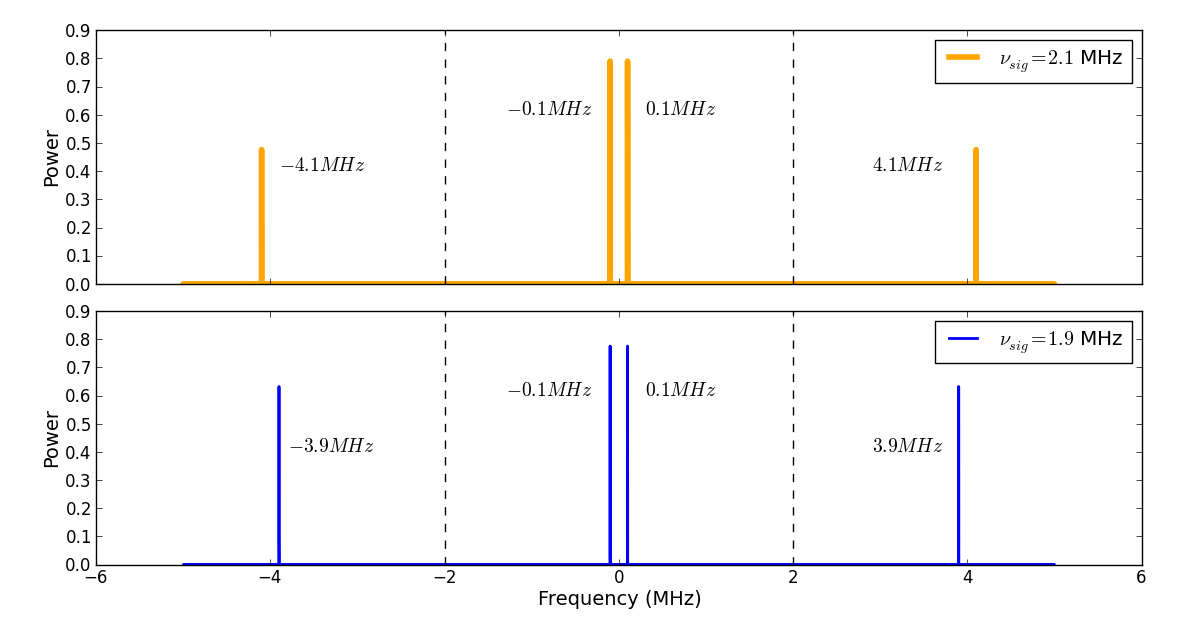
\includegraphics[width=460px]{analogmixing_spectrum}
}
\caption[SODUMB]{Power spectrums of analog mixer output for $\nu_{LO}=2$ MHz (black dotted line), digitally sampled at $10$ MHz. Notice that both results have spectral features at $\pm 0.1 MHz$ due to the fact that the mixers produce frequencies at $\nu_{LO} \pm \nu_{sig}$ as well as $-\nu_{LO} \pm \nu_{sig}$}
\label{fig:analogmixing_spectrum}
\end{figure}

The power spectrum of the mixed signals feature upper and lower sidebands in addition to features at both positive and negative frequencies, as predicted earlier. From Eq. \ref{eq:bands}, the upper sideband (the sum frequency component) occurs at $2\nu_{sig} + \delta$, and the lower sideband (the difference frequency component) occurs at $\delta$.

A small section of the two waveforms are shown in the top row of Figure \ref{fig:analogmixing_signal}. The upper and lower sidebands can be seen by the high frequency oscillations (upper sideband) on top of the slower periodic fluctuation (lower sideband). To filter out the upper sideband and keep only the lower sideband, we can use Fourier filtering.

To do this, we start by zeroing out the sum frequency values in the fourier transform data from Figure \ref{fig:analogmixing_spectrum}. For the $2.1$ MHz case, we will zero out the components around $\pm4.1$ MHz and for the $1.9$ MHz case, we will zero out the components around $\pm3.9$ MHz. We can then apply an inverse discrete Fourier transform and get the waveforms shown in the bottom row of Figure \ref{fig:analogmixing_signal}. These waveforms no longer feature a strong high frequency oscillation; only the slower frequency at $0.1$ MHz remains. Unfortunately, Fourier filtering does not seem to work perfectly at the extreme ends of the time domain when the inverse transform is applied, which is why the plots begin at $100 \mu s$. This is probably due to the fact that the waveform needs to suddenly terminate at the ends which requires frequency components beyond the single frequency we filtered out.

\begin{figure}[H]
\center{
  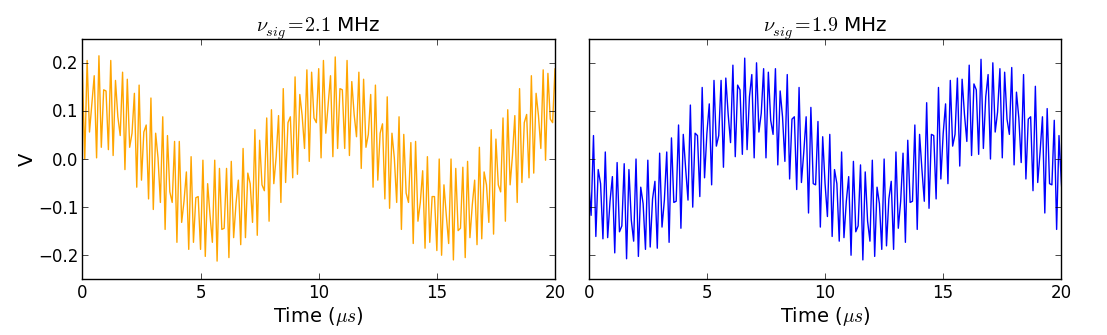
\includegraphics[width=460px]{analogmixing_nofilter}
  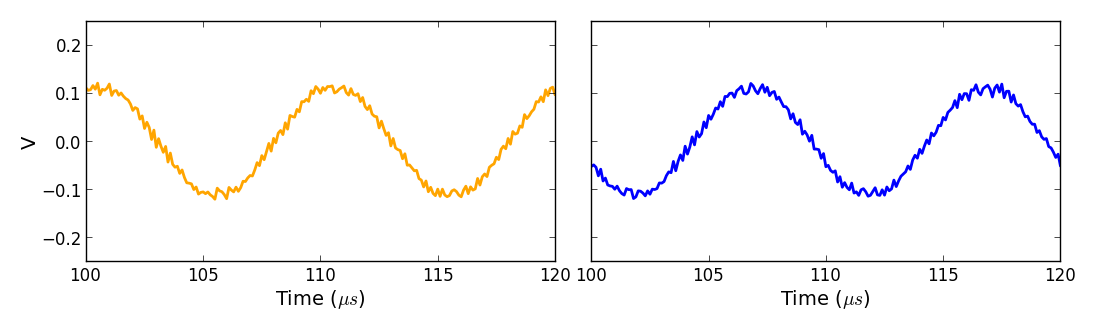
\includegraphics[width=465px]{analogmixing_yesfilter}
}
\caption[SODUMB]{Top: Time domain output from analog mixer with $\nu_{LO}=2$ MHz, digitally sampled at $10$ MHz. The high frequency upper sideband can be seen on top of the slower lower sideband. Bottom: The same waveforms after removing the upper sidebands using Fourier filtering. Only the $0.1$ MHz lower sideband remains.}
\label{fig:analogmixing_signal}
\end{figure}


\subsubsection{Digital Mixing Using the ROACH}
The ROACH (Reconfigurable Open Architecture for Computing Hardware), is a system consisting of a CPU running a Linux kernel and an FPGA, which can be configured to perform tasks with many logic gates running in parallel, synchronized in this lab by a $200$ MHz clock. We can connect to it remotely and configure our data collection by writing to the FPGA's registers. The FPGA writes output data into block random access memory (BRAM). Once the BRAM is full, the data can be copied out of the ROACH for analysis.

\subsubsection{Double Sideband (DSB)}
In the last section, we used an analog mixer to mix our signals with frequency $\nu_{LO}$ and $\nu_{sig}$. The ROACH is capable of digitally mixing the two signals and writing the result to BRAM. If we follow the same procedure as in Section 3.1, this time mixing digitally with the ROACH, we expect to see a similar result. The theory is the same, and the expected output frequencies are still given by Eq. \ref{eq:bands}.

For consistency, we will continue to use a local oscillator frequency of $2$ MHz, and signal frequencies of $2.1$ and $1.9$ MHz. The only difference is that we will clock the ROACH at a rate of $200$ MHz, which is the rate at which logic gates in the FPGA will execute their operations and the rate at which data will be sampled.

The results of digital mixing with these signal frequencies can be seen in Figure \ref{fig:digitalmixing}. The waveform and power spectrum are very similar to the results of the analog mixing case in Figure \ref{fig:analogmixing_spectrum}, with the same spectral features. However, there are a couple differences that can be seen in the power spectrum by noticing that the peaks seem wider than their counterparts in Figure \ref{fig:analogmixing_spectrum}.

\begin{figure}[H]
\center{
  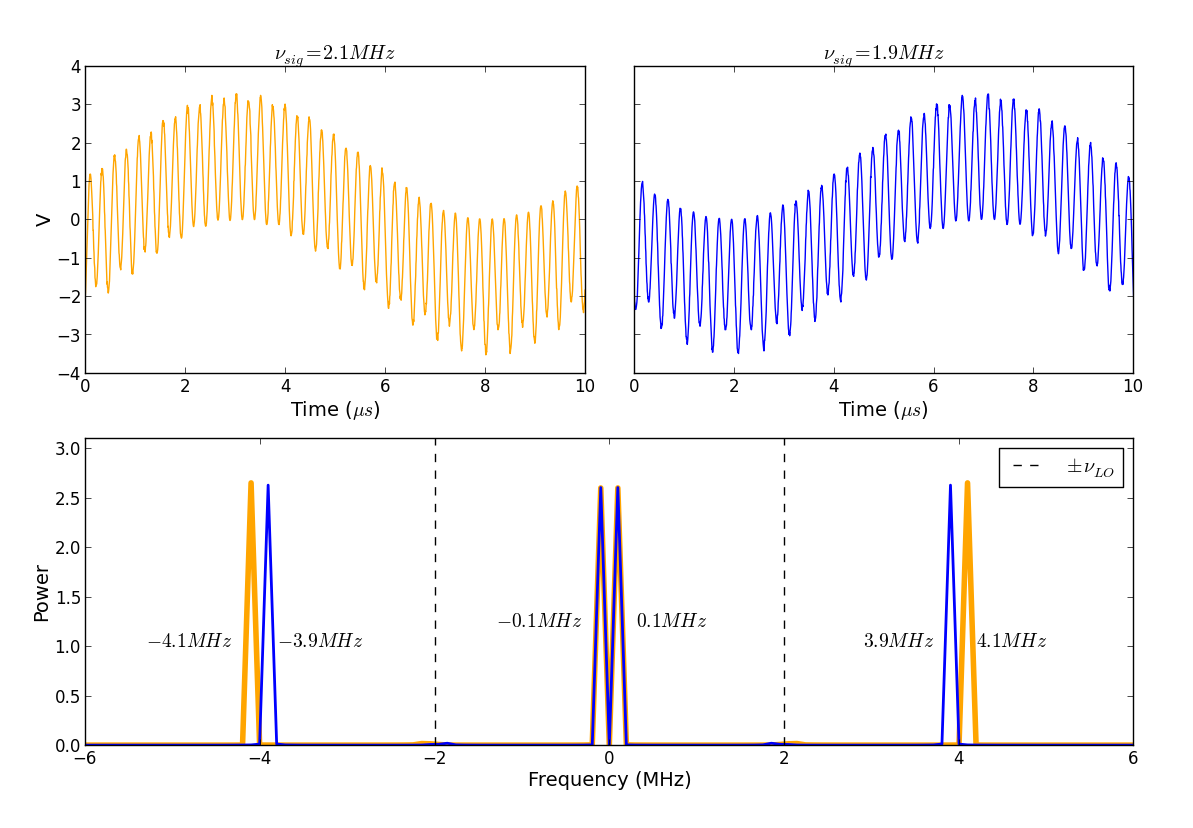
\includegraphics[width=460px]{digitalmixing}
}
\caption[SODUMB]{Similar to Figures \ref{fig:analogmixing_signal} and \ref{fig:analogmixing_spectrum}, this time mixing digitally using the ROACH. Top: Output of digital mixer with $\nu_{LO}=2$ MHz, sampled at $200$ MHz.  Bottom: The power spectrum for both of the outputs. The spectral features occur at the same frequencies as in the analog case of Figure \ref{fig:analogmixing_spectrum}.  We do not observe a DC offset that was predicted by the lab manual. The peaks in the spectrum consist of a single datapoint each---the reason they look wider than in Figure \ref{fig:analogmixing_spectrum} is that the limited size of the ROACH's BRAM only allowed us to sample for about one period, which limited our resolution in the frequency domain.}
\label{fig:digitalmixing}
\end{figure}

The reason for these apparently wider peaks is a lower frequency resolution due to a limited sample size. When data collection is triggered on the ROACH, data points are collected and stored in BRAM until the BRAM is full, limiting the number of data points that we can take. Apparently, the BRAM can only store 2048 32-bit signed integers, meaning if we take samples at $200$ MHz we can sample for $10.24$ $\mu s$. In comparison, when we sampled the output of our analog mixer using the Pulsar card in Section 3.1, we took 16384 values at $10$ MHz, meaning we sampled for $1$ $ms$, one hunderd times longer. Because of this, our resolution in the frequency domain for digitally sampling on the ROACH is one hundred times lower than in the earlier section, which is why the peaks in the spectrum look so wide.

One way to solve this minor issue would be to decrease the clock rate much lower than $200$ MHz, so that the BRAM does not fill up as quickly. This would allow us to take data for a longer period of time.



\subsubsection{Single Sideband (SSB)}
In the DSB cases, both analog and digital, we mixed our signal $f$ with a local oscillator of the form $\cos(\omega t)$. Because the $\cos$ has no imaginary part, we essentially mix our signal with both $e^{j \omega t}$ and $e^{-j \omega t}$ components, creating the upper and lower sidebands, respectively. If instead we wanted to have only a single sideband, we would need to mix our signal with a complex local oscillator of the form $e^{j \omega t}$

Using the ROACH's FPGA, we will be able to mix with both a $\cos$ and $\sin$ wave simultaneously. The FPGA does not output the complex result of the mixing; instead, it mixes the signal simultaneously with samples from a sine and a cosine local oscillator (two sinusoids a quarter period out of phase). These two outputs are stored in separates BRAMs. With those sampled datapoints, we can then programmatically combine them using the following Eq. \ref{eq:mixingexp} to see the full, complex result.
\begin{eqnarray}
Re[f(t) e^{\pm j\omega t}] &=& f(t) \cos(\omega t)\nonumber\\
Im[f(t) e^{\pm j\omega t}] &=& \pm f(t) \sin(\omega t) \nonumber\\
f(t) e^{\pm j\omega t} &=& [f(t) \cos(\omega t)] \pm j [f(t) \sin(\omega t)] \label{eq:mixingexp}
\end{eqnarray}
The frequency of the LO ($\omega$ in Eq. \ref{eq:mixingexp}) is set by the ROACH's sampling clock and the value written to the \texttt{lo\_freq} register, which I will call $x$. To generate samples of a $\cos$ and $\sin$ wave, the FPGA maps the interval of $0$ to $2\pi$ into 256 steps; i.e. $0, \frac{2\pi}{256}, \frac{2\pi}{128}, \frac{2\pi}{64}$, etc. 

Each clock cycle, the ROACH increments its current position in the interval by $x$ steps. The FPGA then evaluates $\cos$ and $\sin$ at that value to be mixed with the next sampled point of the incoming signal. Thus, an entire period of $2\pi$ is completed in $256/x$ steps. With a clock rate of $\nu_{samp}$, the frequency of the LO generated in this fashion is
\begin{eqnarray}
\nu_{LO} = \frac{x}{256} * \nu_{samp} \label{eq:lo_freq}
\end{eqnarray}
Using the above Eq. \ref{eq:lo_freq}, we can determine the local oscillator frequency for any value we write to the FPGA's \texttt{lo\_freq} register.

To demonstrate our SSB mixer, we generate a $6$ MHz, $0$ dBm signal with the SRS and mix it with the LO frequencies listed in the following table, for a $200$ MHz clock rate. Because we want a single sideband mixer that takes only the lower sideband, we will use the version of Eq. \ref{eq:bands} with the minus sign. The signal generated by the SRS will contain both ``positive" and ``negative" frequencies, as it is simply a cosine signal, so we expect to see two frequencies in the output after combining the real and imaginary parts: $\pm \nu_{sig} - \nu_{LO}$. Our Nyquist rate is $100$ MHz, so we should have no problem seeing these signals.
\begin{center}
  \begin{tabular}{ c | c | c }
    $x$ & $\nu_{LO}$ [$MHz$] & $\nu_{output} = \pm \nu_{sig} - \nu_{LO}$ [$MHz$]\\ \hline
    $1$ & $0.782 $ & $-6.782$, $5.218 $ \\
    $2$ & $1.563 $ & $-7.563$, $4.437$\\
    $4$ & $3.125 $ & $-9.125$, $2.875$ \\
    $16$ & $12.5 $ & $-18.5$, $6.5$\\
  \end{tabular}
\end{center}

Figure \ref{fig:ssb} illustrates the result of digitally mixing for the third case, $\nu_{LO} = 3.125 MHz$. As expected, this case has lower side bands at $-9.125$ MHz and $2.875$ MHz. The upper side bands, which would have been at $-2.875$ MHz and $9.125$ MHz, have been avoided by combining both real and imaginary parts of the mixer output.

The power spectrum also includes a small spike at $-3.125$ MHz, the LO frequency. It is about an order of magnitude smaller than the sidebands, so it does not feature prominently in the time domain waveform. We will remove this feature as well as the $-9.125$ MHz sideband using Fourier filtering.

The result of our Fourier filter containing both real and imaginary components is overlaid on Figure \ref{fig:ssb}, isolating the $2.875$ MHz component. This extracted waveform has a positive frequency, which can be seen by noticing the imaginary part (the $\sin$ component) trails the real part by a quarter phase, consistent with a positive frequency. It can also be seen by noticing that $2.875$ MHz is greater than zero.

The primary advantage of SSB mixing is that only one of the two possible sidebands are produced. For a real-valued signal, the output will include two different frequencies, as opposed to four in the DSB case. However, to prevent the unwanted sidebands from sneaking into the output, the real and complex components of the local oscillator must be held at exactly a quarter period out of phase---if they are off of this phase we will start to see the unwanted sideband in the output spectrum.

Because of this phase requirement, it is difficult to implement an \textit{analog} SSB mixer since it is difficult to keep analog signals in perfect phase at many different frequencies. Since the digital version of the SSB uses the ROACH's clock rate to sync the real and imaginary components of the local oscillator, those components will always be at the same frequency and the phase can be adjusted programmatically if they are sligthly off. Another disadvantage to analog mixing is that you can be limited by the bandwidth of the equipment you are using; the ZAD-1's ``L" and `R" ports do not couple to DC or low frequencies of a few kHz.

As far as effort goes, it is much simpler to implement a DSB mixer and then filter out the unwanted frequencies, either digitally or using an analog circuit. Figure \ref{fig:analogmixing_signal} and Figure \ref{fig:ssb} show an analog DSB and digital SSB mixer respectively. Once a Fourier filter is applied, they both extract the desired signal equally well; thus I think it usually would make more sense to implement a simple analog mixer, and deal with filtering out unwanted frequencies after the fact.

\begin{figure}[H]
\center{
  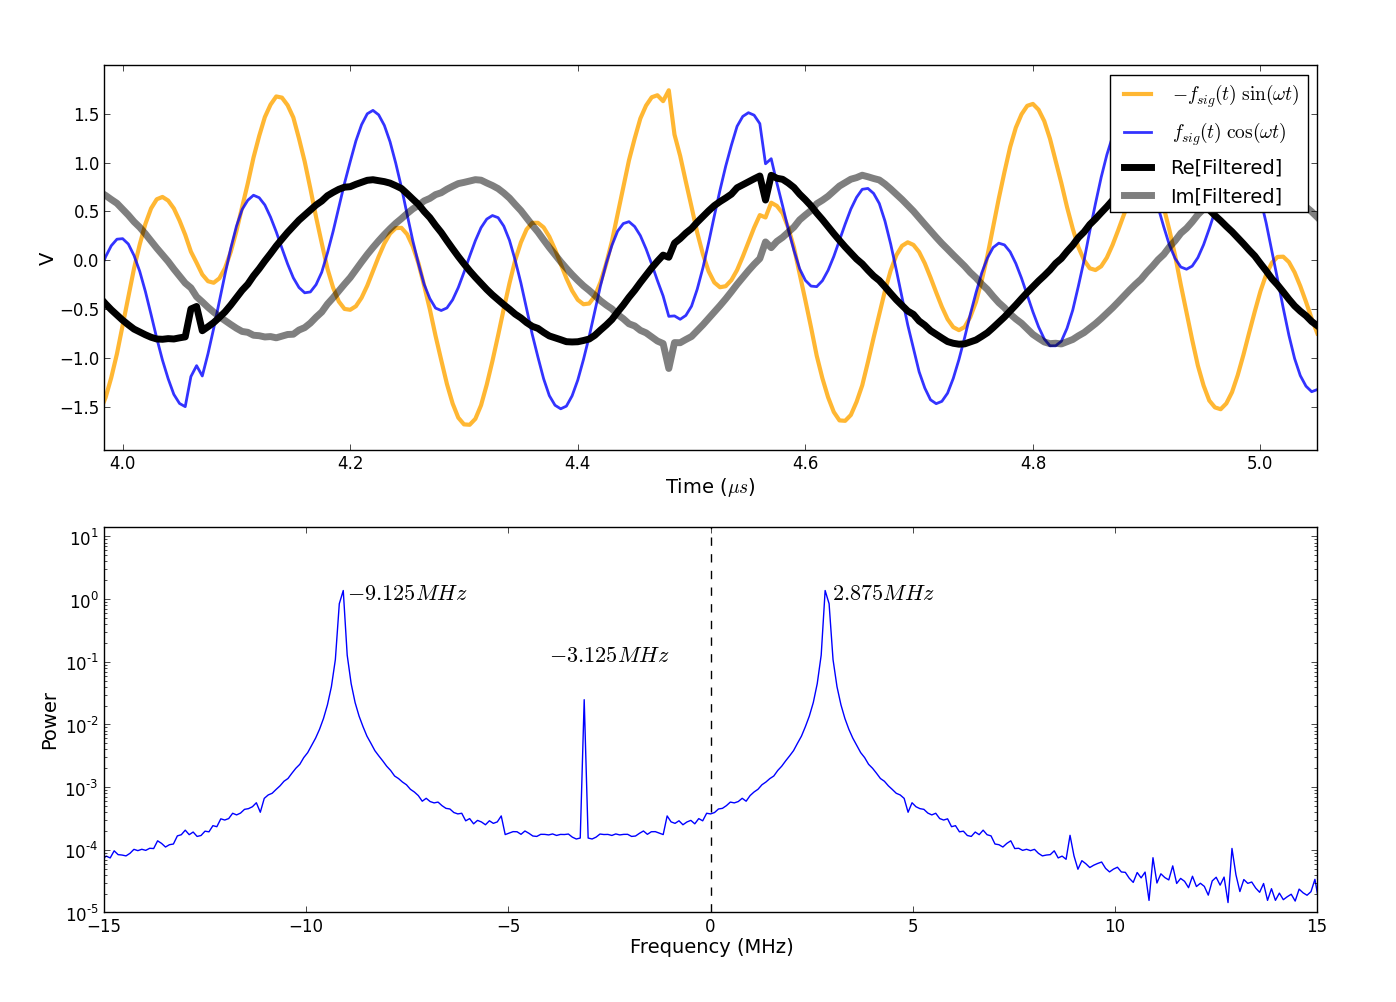
\includegraphics[width=480px]{ssb}
}
\caption[SODUMB]{Top: The result of digitally mixing a $6 MHz$ signal with a $3.125 MHz$ local oscillator. The blue line represents the real part, Re${[f(t)e^{-j\omega t}]} = f(t)\ \cos(\omega t)$, and the orange line represents the imaginary part, Im${[f(t)e^{-j\omega t}]} = -f(t)\ \sin(\omega t)$. Overlaid in a thick black line is the real part of the waveform resulting from using Fourier filtering to remove the $-9.125$ MHz and $-3.125$ MHz components. The thick, lighter, line is the imaginary part of the filtered waveform. Bottom: Power spectrum of the complex waveform. There are clear peaks at $-\nu_{LO} \pm \nu_{sig}$, as well as a small peak at $\nu_{LO}$ from the local oscillator. We filter out the two negative peaks to extract the desired signal.}
\label{fig:ssb}
\end{figure}

\subsection{FIR Filter}
A FIR, or Finite Impulse Response, filter is a way to implement a frequency domain filter by convolving in the time domain. In this section, we implement a FIR filter using the FPGA. The implementation of an FIR filter on the FPGA allows us to convolve an incoming signal with a custom waveform in the time domain \textit{as the signal is sampled}. Our filter has 8 taps, so we choose 8 real and 8 imaginary coefficients to represent the filter, which we tell the FPGA by writing them into its \texttt{coeff} registers. As the signal is sampled, the FPGA multiplies each of the last eight points from the ADC with their corresponding coefficients, and sums them up. Each clock cycle, a new point is sampled and the process is repeated. The sums form a new waveform, and the net effect is that we  essentially drag, or \textit{convolve}, the incoming signal across our filter. The sums are largest at times when the signal ``looks like" our filter, and smallest when the sample does not resemble our filter---thus, the FIR filter picks out portions of the signal most similar to the filter shape.

\subsubsection{Choosing Coefficients}
We use this functionality to implement a bandpass filter. To choose coefficients for the FIR filter, we first create our bandpass in the frequency domain---a square spectrum centered around a certain frequency---and apply the inverse fourier transform to it to get the filter in the time domain. Since we are working digitally, we will only choose 8 points (See Figure \ref{fig:fir}) of the filter so that when we do the inverse discrete fourier transform we wind up with a complex coefficient for each of the eight \texttt{coeff} registers.

Our bandpass in this experiment is a 5/8-band filter, centered around $0$ Hz. Since our clock/sample rate is $200$ MHz, the Nyquist rate is $100$ MHz and the frequency range that we will concern ourselves with is the range $-100$ MHz to $100$ MHz. The 5/8-band filter will be a filter with a full response in 5/8 of that range centered around 0, or from $-62.5MHz$ to $62.5 MHz$. Elsewhere, the filter's response should be zero, as depicted in Figure \ref{fig:fir}. To be able to take the discrete inverse fourier transform of this, we take eight equally spaced samples from the ideal filter and use the inverse discrete Fourier transform algorithm from NumPy's \texttt{fft} module. The points taken in the frequency domain and the corresponding complex coefficients in the time domain are enumerated in the following table:

\begin{center}
  \begin{tabular}{ c | c }
    $\nu$ [MHz] & Power \\ \hline
    $-100$ & $0 $\\
    $-75$ & $0 $\\
    $-50$ & $1 $\\
    $-25$ & $1 $ \\
    $0$ & $1 $\\
    $25$ & $1 $  \\
    $50$ & $1$ \\
    $75$ & $0 $ \\
  \end{tabular}
  $\rightarrow$ [Inverse DFT] $\rightarrow$
  \begin{tabular}{c | l | c }
    t (ns)& Real Coeff. & Imag. Coeff.\\ \hline
    0 & \texttt{0.125} & $0$ \\
    5 & \texttt{-0.0517...}  & $0$ \\
    10 & \texttt{-0.125} & $0$ \\
    15 & \texttt{0.3017...} & $0$ \\
    20 & \texttt{0.625} & $0$ \\
    25 & \texttt{0.3017...} & $0$ \\
    30 & \texttt{-0.125} & $0$ \\
    35 & \texttt{-0.0517...} & $0$ \\
  \end{tabular}
\end{center}


One thing to note is that the imaginary coefficients are all zero. This can be understood by noticing that the 5/8-band filter is symmetric around zero. As we have seen earlier in the lab in our DSB mixers, this symmetry between positive and negative frequency is indicative of a real-valued function.

Since we are using a filter that only convolutes over 8 time steps, we have only fixed our filter's response at the 8 frequencies that we choose. However, the waveform entering the filter can of course contain arbitrary frequency values. To determine the filter's actual expected response as a function of frequency, we can ``pad" the time domain filter with zeroes to increase the amount of time it covers. This way, when we fourier transform our time domain waveform back into the frequency domain, we will have much higher resolution and will see what our filter looks like at frequencies in between the eight discrete points that we chose earlier. The dashed line in Figure \ref{fig:fir} represents this response. This filter contains ripples that do not exist in the ideal filter due to the fact that our discrete inverse Fourier transform over only eight points is not capable of encoding such a high resolution in the frequency domain. To create a \textit{perfect} square filter, one would theoretically have to create a filter that covolutes time steps starting from the beginning of time up until the end of time, and ain't nobody got time for that.
\begin{figure}[H]
\center{
  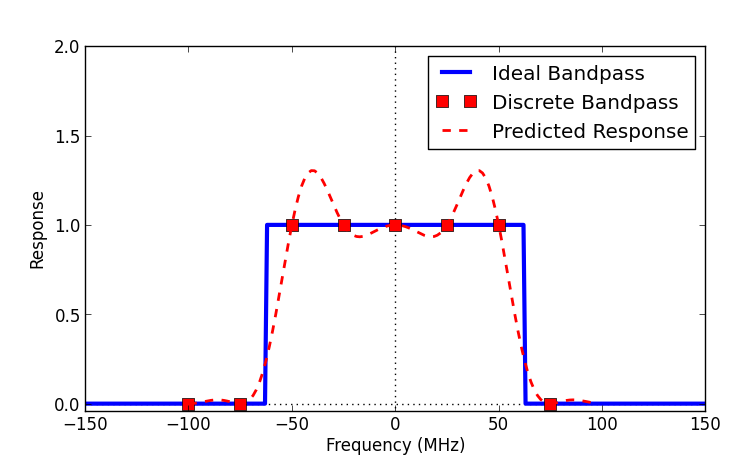
\includegraphics[width=350px]{firfrequency}
}
\center{
  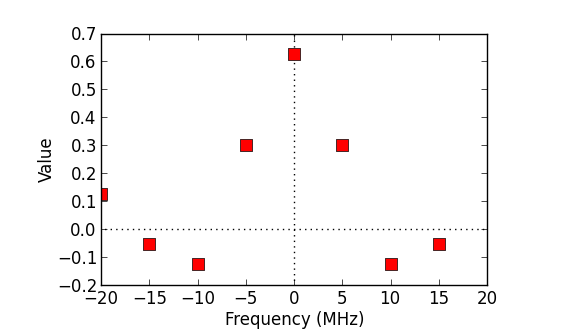
\includegraphics[width=250px]{firtime}
}
  
\caption[SODUMB]{Top: Ideal bandpass filter with the 8 discrete values used in the FIR filter marked as squares. The actual response of a filter that uses only those 8 points is shown as a dashed line. Bottom: The inverse fourier transform of those 8 points. They follow the shape of a sinc function ($\frac{\sin{x}}{x}$).}
\label{fig:fir}
\end{figure}

\subsubsection{Testing Filter Response}
To test our FIR filter's response as a function of frequency, we want to compare how the power spectrum of a waveform looks with and without the filter applied. For purposes of this experiment, the response of the filter at a frequency $\nu$ is the ratio of the power at that frequency with the filter to the power at that frequency without the filter, $P_{filtered}/P_{unfiltered}$. For example, If the power spectrum has a large spike at a frequency $10$ MHz without the filter, but a spike half as large at $10$ MHz with the filter, then the response of the filter at $10$ MHz is $0.5$. 

The way we can see the expected magnitude in the power spectrum is by using the FIR filter with all coefficients set to zero except for one set to the maximal possible value (a close to one as possible). This essentially reproduces the original signal as output because the FIR is simply convoluting the incoming signal with a delta function of magnitude 1---each point of the incoming signal is simply recreated in the output as it is ``dragged" across the delta function filter.

To probe many frequencies in our range of $-100$ MHz to $100$ MHz, we use the digital SSB mixing techniques of the previous section. The SRS Signal Generator can only produce signals up to $30$ MHz; thus, to get larger signal frequencies we will mix our signal with LO frequencies that will produce upper and lower sidebands to span this range.

We use a $25$ MHz signal at $0$ dBm, mixed with LO frequencies ranging from $5$ MHz to $50$ MHz. Since we will combine real and imaginary parts programmatically, we can add them in both forms described by Eq. \ref{eq:mixingexp} to produce upper and lower sidebands.

After collecting these mixed waveforms with and without the FIR filter applied, we square the magnitude of the DFT of our convolved waveform to get the power spectrum. Each sideband that we create, enumerated in the upcoming table, represents a single datapoint at which the response is the ratio of the filtered spike's size to the unfiltered spike's size.

\begin{center}
  \begin{tabular}{c | c | c }
    LO Freq. [MHz] & Upper Sidebands [MHz] & Lower Sidebands [MHz] \\ \hline
    3.125 & 28.125, -21.875 & 21.875, -28.125 \\
    12.5 & 37.5, -12.5 & 12.5, -37.5 \\
    25.0 & 50.0, 0.0 & 0.0, -50.0 \\
    31.25 & 56.25, 6.25 & -6.25, -56.25 \\
    35.9375 & 60.9375, 10.9375 & -10.9375, -60.9375 \\
    37.5 & 62.5, 12.5 & -12.5, -62.5 \\
    39.0625 & 64.0625, 14.0625 & -14.0625, -64.0625 \\
    43.75 & 68.75, 18.75 & -18.75, -68.75 \\
    50.0 & 75.0, 25.0 & -25.0, -75.0 \\
    \end{tabular}
\end{center}

For each of these LO settings, we collect data twice---once with the coefficients for our 5/8-band filter, and again with all coefficients zero except for one (to normalize the output strength).

We take the ratio $P_{filtered} / P_{unfiltered}$ at all these frequencies, and get the results in Figure \ref{fig:firresponse}. They follow very closely to the predicted response, which is to be expected because the filtering and mixing was all done digitally. The fact that the response matches expectation well is still very apparent.
\begin{figure}[H]
\center{
  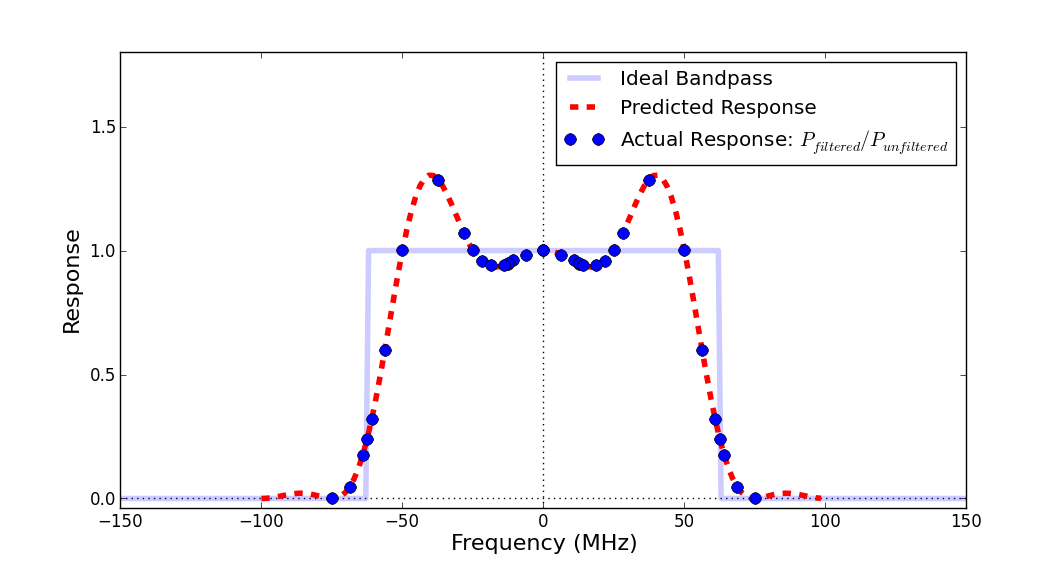
\includegraphics[width=450px]{firresponse}
} 
\caption[SODUMB]{The response of our 5/8-band filter implemented using the 8 tap FIR filter. The ideal 5/8-band filter in overlaid in light blue, and the theoretical response of the eight tap filter as a function of frequency is in red.}
\label{fig:firresponse}
\end{figure}

\section{Conclusion}

In testing the Nyquist criterion, we find that signals of all frequencies up to one-half the sampling rate can be sampled successfully. Though sampling faster can produce a more faithful representation of a signal in the time domain, there is not a huge difference in the frequency domain representation of the signal (the power spectrum) for faster sampling rates. In practical application, it may be most economical to sample as slowly as possible without violating the Nyquist limit, since the spectral information will be preserved while keeping the data files smaller. However, one should avoid sampling at \textit{exactly} the Nyquist frequency as the potential for a misleading ``flat" waveform is possible in this case.

Additionally, explored both analog and digital methods of DSB and SSB mixing and were able to compare the advantages and disadvantages of each. We find that it is possible to implement a SSB mixer digitally but it is more complicated and requires more resources than an analog DSB mixer. The output of the analog DSB can be filtered using techniques like Fourier filtering in order to extract a comparable result to that of the SSB method. 

Finally, the FIR filter.



\section{Acknowledgement}
I would like to thank my lab partners Maissa and Sal for their work in getting us through this lab. Also thanks to the lab instructors Aaron Parsons, Karto Keating, and Baylee Bordwell for teaching us the lab material, helping us with debugging the ROACH, and sustaining us with baked goods. Especially to Karto for providing us with with the now defunct \texttt{set\_srs}, which automagically just worked data collection so much easier.
All figures were done in Python using the Numpy and Matplotlib libraries.

\section{Appendix}
\subsection{Converting FIR Coefficients to Binary}
When implementing a FIR filter, the FPGA reads 18 bit\footnote{The register holds 32 bits but only 18 bits are used.}, fixed point, 2's complement numbers from the \texttt{coeff} registers, with 17 digits after the binary point. The smallest bit, therefore, will represent the value $2^{-17}$, and the range of values that can be represented go from $-1$ to $1-2^{-17}$. A easy way to convert a decimal value into this odd representation is to divide that number by $2^{-17}$, and then fill in the preceding bits with zeroes up to the full 32 bits.

This table shows the coefficients\footnote{I truncated the decimal for sake of space. However, the coefficients were determined using \texttt{np.fft} with floating point precision; the binary and hex columns include as much precision as NumPy was willing to offer.} we wanted to use in our 5/8-band filter, as well as their binary representation in this representation and their hexadecimal representation.

\begin{center}
  \begin{tabular}{ l | c | c }
    Coeff. & Binary & Hex\\ \hline
    \texttt{-0.0517...}  &  \texttt{1.11110010101111101} & \texttt{0x3e57d}\\
    \texttt{-0.125} &  \texttt{1.11100000000000000} & \texttt{0x3c000}\\
    \texttt{0.125} & \texttt{0.00100000000000000} & \texttt{0x04000}\\
    \texttt{0.3017...} &  \texttt{0.01001101010000010} & \texttt{0x09a82}\\
    \texttt{0.625} &  \texttt{0.10100000000000000} & \texttt{0x14000}\\
   \end{tabular}
\end{center}

\end{document}